\documentclass[11pt,letterpaper]{article}
\usepackage{proposal}
\usepackage{times}
\usepackage{latexsym}
\usepackage{amsmath}
\usepackage{graphicx}
\usepackage[margin=1in]{geometry}

\newcommand{\argmax}[1]{\underset{#1}{\operatorname{argmax}}}

\usepackage{color}

\newcommand{\remove}[1]{}
\newcommand{\Note}[1]{}
%\newcommand{\Note}[1]{\textbf{\large\textcolor{blue}{[#1]}}}
\newcommand{\NoteJS}[1]{\Note{#1~--JS}}

\title{Parallel Sentence Discovery for Low-Resource Languages}

\author{Jason Smith\\
  Center for Language and Speech Processing\\
  Johns Hopkins University\\
  3400 N. Charles St.\\
  Baltimore, MD 21218, USA\\
  {\tt jsmith@cs.jhu.edu}\\
  {\em Advisors:} Chris Callison-Burch, Adam Lopez
}

\begin{document}
\maketitle
\begin{abstract}
One of the most important factors in the performance of a statistical machine
translation (SMT) system is the amount and quality of parallel data it is
trained on. This has motivated work in which parallel sentences are extracted
from document pairs that are not necessarily translations of each other.
Collections of such semi-parallel documents are called comparable corpora. In
this work, we aim to extract parallel sentences from comparable corpora using a
minimal amount of supervision.
\end{abstract}

\section{Introduction}
Almost all modern SMT systems are trained using a large collection of translated
sentence pairs known as a parallel corpus. Sources of parallel data include
parliament proceedings, books, and news articles.
While this data may be abundant for some language pairs, such as
French/English, it is scarce for most others. In addition, even when parallel
data is available, it may not match the domain of the data you wish to
translate, and this can have a large effect on performance \cite{Munteanu05}.

The creation of new parallel corpora can be expensive, especially when bilingual
speakers are rare for the language pair of interest.
\NoteJS{maybe show numbers for this if available}
In order to acquire more parallel data without costly human annotation,
researchers have looked to corpora which may contain some parallel sentences,
but are not completely parallel. Such corpora are referred to as comparable
corpora, and examples include multilingual news feeds \cite{Munteanu05} and
Wikipedia articles \cite{Adafre06,Smith10}. 
Most work in extracting parallel sentences from
these corpora assumes an initial bilingual dictionary or an existing parallel
corpus.

On the other hand, there has also been work on aligning sentences in parallel
corpora where the documents may contain $2:1$ or $1:2$ sentence alignments, or
there may be large insertions or deletions of sentences \cite{Gale93,Chen93,Moore02}.
This work, by contrast, does not require existing parallel data or a
bilingual dictionary for the language pair of interest. Instead, the structure
of the documents and the lengths of the sentences are used to determine the
sentence alignment. Any information about bilingual word correspondence comes
from the parallel data that is being aligned.

In this work, we aim to combine techniques from both parallel and comparable
sentence alignment to improve the state of the art for parallel sentence
extraction from comparable corpora. First, we will describe a novel
discriminative model for aligning sentences in comparable documents.
We will also describe a model for aligning comparable documents which
needs only a minimal amount of supervision. Similar to how unsupervised word
alignment models can learn their parameters from unlabeled data, we aim to learn
parameters for a sentence alignment model from comparable unaligned documents.

\section{Sentence Alignment}
In this section, we will describe our task and notation.
We will view both parallel corpora alignment and the extraction of parallel
sentences from comparable corpora as an alignment task. In either type of
alignment we are given a set of bilingual document pairs in {\em source} and {\em
target} languages. When performing parallel corpora alignment, these document
pairs will correspond to each other very strongly, while in the case of
comparable corpora, some these document pairs may contain no parallel sentences.
\newcite{Munteanu05} take their document pairs from news stories published at
roughly the same time, while \newcite{Adafre06,Smith10} use entries from
Wikipedia that are on the same topic (Figure \ref{fig:wiki} gives and example).
The task of finding comparable document pairs is not addressed in this work.

\begin{figure*}[ht]
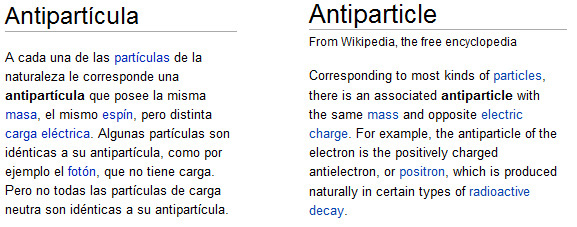
\includegraphics[width=\textwidth]{images/wiki.jpg}
\caption{An example of a Spanish/English document pair from Wikipedia.}
\label{fig:wiki}
\end{figure*}

Each document pair contains a sequence of source sentences (denoted by ${\bf
S}$) and target sentences (denoted by ${\bf T}$). Individual source and target
sentences are referred to by $S$ and $T$ respectively. Similarly, we refer to
the words within source and target sentences with the lowercase $s$ and $t$. We
borrow the notation of \cite{Och03} for describing alignments between sentences
as subsets of the Cartesian product of sentence positions. Sentence alignments
are referred to with the uppercase $A$, and word alignments with the lowercase
$a$.

The goal of sentence alignment is to identify which sentence pairs in the
bilingual document pairs are parallel. We view this as a retrieval task for
parallel sentence pairs, and so when annotated sentence alignments are present,
we can compute precision, recall, and F-measure.

\section{Discriminative Sentence Alignment}
\label{sec:disc}
In this section we will describe a discriminative model for performing sentence
alignment on comparable document pairs.
We use Wikipedia as our source for
comparable documents.

\subsection{Wikipedia as a Comparable Corpus}
\label{sec:wiki}
Wikipedia \cite{wikipedia} is an online collaborative encyclopedia available in
a wide variety of languages.  While the English Wikipedia is the largest, with
over 3 million articles, there are 24 language editions with at least 100,000
articles.

Articles on the same topic in different languages are also connected via
``interwiki'' links, which are annotated by users.  This is an extremely
valuable resource when extracting parallel sentences, as the document alignment
is already provided.  
Table \ref{table:interwiki} shows how
many of these ``interwiki'' links are present between the English Wikipedia and the
16 largest non-English Wikipedias.

\begin{table*}
\begin{center}
\begin{tabular}{|c|c|c|c|c|c|c|c|}
\hline
French & German & Polish & Italian & Dutch & Portuguese & Spanish & Japanese \\
496K & 488K & 384K & 380K & 357K & 323K & 311K & 252K\\
\hline
Russian & Swedish & Finnish & Chinese & Norwegian & Volap\"{u}k & Catalan & Czech \\
232K & 197K & 146K & 142K & 141K & 106K & 103K & 87K\\
\hline
\end{tabular}
\end{center}
\caption{Number of aligned bilingual articles in Wikipedia by language (paired with English).}
\label{table:interwiki}
\end{table*}

Wikipedia's markup contains other useful indicators for parallel sentence
extraction.  The many hyperlinks found in articles have previously been used as
a valuable source of information.  \cite{Adafre06} use matching
hyperlinks to identify similar sentences.  Two links match if the articles they
refer to are connected by an ``interwiki'' link.
Also, images in Wikipedia are often stored in a central source across
different languages; this allows identification of captions which may be
parallel.  Finally, there are other minor forms
of markup which may be useful for finding similar content across languages, such
as lists and section headings.  In Section \ref{sec:features}, we will explain
how features are derived from this markup.

\subsection{Models for Parallel Sentence Extraction}
\label{sec:models} In this section, we will focus on methods for
extracting parallel sentences from aligned, comparable documents.
The related problem of automatic document alignment in news and
web corpora has been explored by a number of researchers,
including
\newcite{Resnik03}, \newcite{Munteanu05},
\newcite{Tillmann09a}, and \newcite{Tillmann09b}.
Since our corpus already contains document alignments, we sidestep
this problem, and will not discuss further details of this issue.
That said, we believe that our methods will be effective in
corpora without document alignments when combined with one of the
aforementioned algorithms.


\subsubsection{Binary Classifiers and Rankers}
Much of the previous work involves building a binary classifier for sentence
pairs to determine whether or not they are parallel
\cite{Munteanu05,Tillmann09a}.
The training data usually comes from a standard parallel corpus.  There is a
substantial class imbalance ($O(n)$ positive examples, and $O(n^2)$
negative examples), and various heuristics are used to mitigate this problem.
\newcite{Munteanu05} filter out negative
examples with high length difference or low word overlap (based on a bilingual
dictionary).

We propose an alternative approach: we learn a ranking model, which, for each sentence in the {\em
source} document, selects either a sentence in the {\em target} document that it is
parallel to, or ``null''.
This formulation of the problem avoids the class imbalance issue of the binary classifier.

In both the binary classifier approach and the ranking approach, we use a Maximum Entropy
classifier, following \newcite{Munteanu05}.

\subsubsection{Sequence Models}
In Wikipedia article pairs, it is common for parallel sentences to
occur in clusters.  A global sentence alignment model is
able to capture this phenomenon. For both parallel and comparable
corpora, global sentence alignments have been used, though the
alignments were monotonic
\cite{Gale93,Moore02,Zhao02}.
Our model is a first order linear chain Conditional Random Field
(CRF) \cite{Lafferty01}. The set of source and
target sentences are observed. For each {\em source} sentence, we
have a hidden variable indicating the corresponding {\em target}
sentence to which it is aligned (or null). The model is similar to the
discriminative CRF-based word alignment model of
\cite{Blunsom06}.

\subsubsection{Features}
\label{sec:features}
Our features can be grouped into four categories.

\subsubsection*{Features derived from word alignments}
%kristina-edit-1

We use a feature set inspired by \cite{Munteanu05}, who defined
features primarily based on IBM Model 1 alignments
\cite{Brown93}.  We also use HMM word alignments
\cite{Vogel96} in both directions ({\em source} to {\em target} and
{\em target} to {\em source}), and extract the following features based on these
four alignments:\footnote{These are all derived from the one best alignment, and
normalized by sentence length.}

\begin{enumerate}
\item Log probability of the alignment
\item Number of aligned/unaligned words
\item Longest aligned/unaligned sequence of words
\item Number of words with fertility 1, 2, and 3+
\end{enumerate}

We also define two more features which are independent of word alignment
models.  One is a sentence length feature taken from \cite{Moore02}, which
models the length ratio between the {\em source} and {\em target} sentences with
a Poisson distribution.  The other feature is the difference in relative
document position of the two sentences, capturing the idea that the aligned
articles have a similar topic progression.

The above features are all defined on sentence pairs, and are included in the
binary classifier and ranking model.
\subsubsection*{Distortion features} In the sequence model, we use additional distortion
features, which only look at the difference between the position
of the previous and current aligned sentences.  One set of
features bins these distances; another looks at the
absolute difference between the expected position (one after the
previous aligned sentence) and the actual position.

\subsubsection*{Features derived from Wikipedia markup}

Three features are derived from Wikipedia's
markup. The first is the number of matching links in the sentence
pair. The links are weighted by their inverse frequency in the
document, so a link that appears often does not contribute much to
this feature's value.  The image feature fires whenever two
sentences are captions of the same image, and the list feature
fires when two sentences are both items in a list.  These last two
indicator features fire with a negative value when the feature
matches on one sentence and not the other.

None of the above features fire on a null alignment, in either the
ranker or CRF.  There is also a bias feature for these two models, which
fires on all non-null alignments.

\subsubsection*{Word-level induced lexicon features}
In order to address sparsity issues in our seed parallel corpora, we introduce a
bilingual lexicon model which learns word translation probabilities from the
linked Wikipedia articles. The details of this model and the features derived
from it can be found in \cite{Smith10}.

\subsection{Experiments}
\label{sec:exp}

\subsubsection{Data}
We annotated twenty Wikipedia article pairs for three language pairs: Spanish-English,
Bulgarian-English, and German-English.
Each sentence in the {\em source} language was annotated with
possible parallel sentences in the {\em target} language (the target language was
English in all experiments).  The pairs were annotated with a quality level:
{\bf 1} if the sentences contained some parallel fragments, {\bf 2} if the sentences
were mostly parallel with some missing words, and {\bf 3} if the sentences appeared to be direct
translations.  In all experiments, sentence pairs with quality {\bf 2} or {\bf 3} were
taken as positive examples. 

\begin{table*}[ht]
\begin{center}
\begin{tabular}{|c||c|c|c||c|c|c||c|c|c|}
\hline
Language Pair     & \multicolumn{3}{|c||}{Binary Classifier} & \multicolumn{3}{|c||}{Ranker} & \multicolumn{3}{|c|}{CRF} \\
\hline
                  & Avg Prec & R@90 & R@80
                  & Avg Prec & R@90 & R@80
                  & Avg Prec & R@90 & R@80 \\
\hline
\footnotesize{English-Bulgarian} & 75.7  & 33.9  & 56.2    & 76.3  & 38.8  & 57.0    & {\bf 80.6}  & {\bf 52.9}  & {\bf 59.5} \\
\footnotesize{English-Spanish}   & 90.4  & 81.3  & 87.6    & 93.4  & 81.0  & 84.5    & {\bf 94.7}  & {\bf 87.6}  & {\bf 90.2} \\
\footnotesize{English-German}    & 61.8  &  9.4  & 27.5    & 66.4  & 25.7  & 42.4    & {\bf 78.9}  & {\bf 52.2}  & {\bf 54.7} \\
\hline
\end{tabular}
\end{center}
\caption{Average precision, recall at 90\% precision, and recall at 80\%
precision for each model in all three language pairs.  In these experiments, the
Wikipedia features and lexicon features are omitted.}
\label{table:modelcompare}
\end{table*}

\begin{table*}[ht]
\begin{center}
\begin{tabular}{|c||c|c|c||c|c|c|}
\hline
Setting           & \multicolumn{3}{|c||}{Ranker} & \multicolumn{3}{|c|}{CRF} \\
\hline
                  & Avg Prec & R@90 & R@80
                  & Avg Prec & R@90 & R@80\\
\hline
English-Bulgarian & & & & & & \\
\hline
One Direction          & 76.3  & 38.8  & 57.0    & 80.6  & 52.9  & 59.5 \\
Intersected            & 78.2  & 47.9  & 60.3    & 79.9  & 38.8  & 57.0 \\
Intersected +Wiki      & 80.8  & 39.7  & 68.6    & 82.1  & 53.7  & 62.8 \\
Intersected +Wiki +Lex & 89.3  & 64.4  & 79.3    & {\bf 90.9}  & {\bf 72.0}  & {\bf 81.8} \\
\hline
English-Spanish & & & & & & \\
\hline
One Direction          & 93.4  & 81.0  & 84.5    & 94.7  & 87.6  & 90.2 \\
Intersected            & 94.3  & 82.4  & 89.0    & 95.4  & 88.5  & 91.8 \\
Intersected +Wiki      & 94.5  & 82.4  & 89.0    & 95.6  & 89.2  & 92.7 \\
Intersected +Wiki +Lex & 95.8  & 87.4  & 91.1    & {\bf 96.4}  & {\bf 90.4}  & {\bf 93.7} \\
\hline
English-German & & & & & & \\
\hline
One Direction          & 66.4  & 25.7  & 42.4    & 78.9  & 52.2  & 54.7 \\
Intersected            & 71.9  & 36.2  & 43.8    & 80.9  & 54.0  & 67.0 \\
Intersected +Wiki      & 74.0  & 38.8  & 45.3    & 82.4  & 56.9  & {\bf 71.0} \\
Intersected +Wiki +Lex & 78.7  & 46.4  & 59.1    & {\bf 83.9}  & {\bf 58.7}  & 68.8 \\
\hline
\end{tabular}
\end{center}
\caption{Average precision, recall at 90\% precision, and recall at 80\%
precision for the Ranker and CRF in all three language pairs.  ``+Wiki''
indicates that Wikipedia features were used, and ``+Lex'' means the lexicon
features were used.}
\label{table:featurecompare}
\end{table*}



For our seed parallel data, we used the Europarl corpus
\cite{Koehn05} for Spanish and German and the
JRC-Aquis corpus for Bulgarian, plus the article titles for
parallel Wikipedia documents, and translations available from
Wiktionary entries.\footnote{Wiktionary is an online collaborative
dictionary, similar to Wikipedia.} %kristina-edit

\subsubsection{Intrinsic Evaluation}
Using 5-fold cross-validation on the 20 document pairs for each
language condition, we compared the binary classifier, ranker, and
CRF models for parallel sentence extraction. To tune for 
precision/recall, we used minimum Bayes risk decoding.  We define
the loss $L(\tau,\mu)$ of picking target sentence $\tau$ when the
correct target sentence is $\mu$ as $0$ if $\tau=\mu$, $\lambda$ if
$\tau = \textsc{null}$ and $\mu\ne\textsc{null}$, and $1$ otherwise.
By modifying the null loss $\lambda$, the precision/recall
trade-off can be adjusted.  For the CRF model, we used posterior
decoding to make the minimum risk decision rule tractable. As a
summary measure of the performance of the models at different
levels of recall we use average precision as defined in
\cite{Ido06}. We also report recall at precision of 90 and
80 percent. %kristina-edit 
 Table \ref{table:modelcompare} compares the
different models in all three language pairs.

In our next set of experiments, we looked at the effects of the Wikipedia
specific features.  Since the ranker and CRF are asymmetric models,
we also experimented with running the models in both directions and combining
their outputs by intersection.  These results are shown in Table \ref{table:featurecompare}.

Identifying the agreement between two asymmetric models is a commonly
exploited trick elsewhere in machine translation. It is mostly effective
here as well, improving all cases except for the Bulgarian-English CRF where
the regression is slight. More successful are the Wikipedia features, which
provide an auxiliary signal of potential parallelism.

The gains from adding the lexicon-based features can be dramatic
as in the case of Bulgarian (the CRF model average precision
increased by nearly 9 points). The lower gains on Spanish and
German may be due in part to the lack of language-specific
training data. These results are very promising and
motivate further exploration. We also note that this
is perhaps the first successful practical application of an
automatically induced word translation lexicon.

\subsubsection{SMT Evaluation}

We also present results in the context of a full machine translation system
to evaluate the potential utility of this data.  A standard
phrasal SMT system \cite{Koehn03} serves as our testbed, using
a conventional set of models: phrasal models of source given target and
target given source; lexical weighting models in both directions, language
model, word count, phrase count, distortion penalty, and a lexicalized
reordering model.  Given that the extracted Wikipedia data takes the
standard form of parallel sentences, it would be easy to exploit this same
data in a number of systems.

\begin{table*}[ht]
\begin{center}
\begin{tabular}{|rr||r|r||r|r||r|r|}
\hline
      &                & German        & English       & Spanish       & English      & Bulgarian    & English   \\
\hline
      & sentences     & 924,416       & 924,416       & 957,884       & 957,884      & 413,514      & 413,514   \\
\textbf{Medium} \
      & types     & 351,411       & 320,597       & 272,139       & 247,465      & 115,756      & 69,002    \\
      & tokens    & 11,556,988    & 11,751,138    & 18,229,085    & 17,184,070   & 10,207,565   & 10,422,415\\
\hline
      & sentences      & 6,693,568     & 6,693,568     & 7,727,256     & 7,727,256    & 1,459,900    & 1,459,900 \\
\textbf{Large} \
      &      types     & 1,050,832     & 875,041       & 1,024,793     & 952,161      & 239,076      & 137,227   \\
      &      tokens    & 100,456,622   & 96,035,475    & 155,626,085   & 137,559,844  & 29,741,936   & 29,889,020\\
\hline
      & sentences      & 1,694,595     & 1,694,595     & 1,914,978     & 1,914,978    & 146,465      & 146,465   \\
\textbf{Wiki}  \
      &      types     & 578,371       & 525,617       & 569,518       & 498,765      & 107,690      & 74,389    \\
      &      tokens    & 21,991,377    & 23,290,765    & 29,859,332    & 28,270,223   & 1,455,458    & 1,516,231 \\
\hline
\end{tabular}
\end{center}
\caption{Statistics of the training data size in all three language pairs.}
\label{table:mtTrainStats}
\end{table*}

\begin{table*}[ht]
\begin{center}
\begin{tabular}{|rr||r|r||r|r||r|r|}
\hline
      &                & German        & English       & Spanish       & English      & Bulgarian     & English   \\
\hline
\textbf{Dev A} \
      & sentences      & 2,000         & 2,000         & 2,000         & 2,000        & 2,000         & 2,000     \\
      & tokens    & 16,367        & 16,903        & 24,571        & 21,493       & 39,796        & 40,503    \\
\hline
\textbf{Test A}\
      & sentences      & 5,000         & 5,000         & 5,000         & 5,000        & 2,473         & 2,473     \\
      & tokens    & 42,766        & 43,929        & 68,036        & 60,380       & 52,370        & 52,343    \\
\hline
\textbf{Wikitest}\
      & sentences    & 500           & 500           & 500           & 500          & 516           & 516       \\
      & tokens    & 8,235         & 9,176         & 10,446        & 9,701        & 7,300         & 7,701     \\
\hline
\end{tabular}
\end{center}
\caption{Statistics of the test data sets.}
\label{table:mtTestStats}
\end{table*}

For each language pair we explored two training conditions.  The
``Medium'' data
condition used easily downloadable corpora: Europarl for German-English and
Spanish-English, and JRC/Acquis for Bulgarian-English.  Additionally we
included titles of all linked Wikipedia articles as parallel sentences in
the medium data condition.  The ``Large'' data condition includes all the
medium
data, and also includes using a broad range of available sources such as
data scraped from the web~\cite{Resnik03}, data from the United
Nations, phrase books, software documentation, and more.

In each condition, we explored the impact of including additional
parallel sentences automatically extracted from Wikipedia in the
system training data. For German-English and Spanish-English, we
extracted data with the null loss adjusted to
achieve an estimated precision of 95 percent, and for
English-Bulgarian a precision of 90 percent. %kristina-edit-1
Table~\ref{table:mtTrainStats} summarizes the characteristics of
these data sets.  We were pleasantly surprised at the amount of
parallel sentences extracted from such a varied comparable corpus.
Apparently the average Wikipedia article contains at least a
handful of parallel sentences, suggesting this is a very fertile
ground for training MT systems.

The extracted Wikipedia data is likely to make the greatest impact on broad
domain test sets -- indeed, initial experimentation showed little BLEU gain
on in-domain test sets such as Europarl, where out-of-domain training data
is unlikely to provide appropriate phrasal translations.  Therefore, we
experimented with two broad domain test sets.

First, Bing Translator provided a sample of translation
requests along with translations in German-English and
Spanish-English -- this constituted our standard development and
test set for those language pairs.  Unfortunately no such tagged
set was available in Bulgarian-English, so we held out a portion
of the large system's training data to use for development and
test. In each language pair, the test set was split into a
development portion (``Dev A'') used for minimum error rate
training~\cite{OchMert03} and a test set (``Test A'') used
for final evaluation.

\begin{table*}[ht!]
\begin{center}
\begin{tabular}{|lr||l||l|l|}
\hline
Language pair     & Training data     & Dev A             & Test A            & Wikitest     \\
\hline
Spanish-English   & Medium            & 32.6              & 30.5              & 33.0         \\
                  & Medium+Wiki       & 36.7 (+4.1)       & 33.8 (+3.3)       & 39.1 (+6.1)  \\
                  & Large             & 39.2              & \textbf{37.4}     & 38.9         \\
                  & Large+Wiki        &\textbf{39.5} (+0.3)&37.3 (-0.1)       & \textbf{41.1} (+2.2)  \\
\hline
German-English    & Medium            & 28.7              & 26.6              & 13.0         \\
                  & Medium+Wiki       & 31.5 (+2.8)       & 29.6 (+3.0)       & 18.2 (+5.2)  \\
                  & Large             & \textbf{35.0}     & 33.7              & 17.1         \\
                  & Large+Wiki        & 34.8 (-0.2)       &\textbf{33.9} (+0.2)&\textbf{20.2} (+3.1)  \\
\hline
Bulgarian-English & Medium            & 36.9              & 26.0              & 27.8         \\
                  & Medium+Wiki       & 37.9 (+1.0)       & 27.6 (+1.6)       & 37.9 (+10.1) \\
                  & Large             &\textbf{51.7}      &\textbf{49.6}      & 36.0         \\
                  & Large+Wiki        &\textbf{51.7}(+0.0)& 49.4 (-0.2)       &\textbf{39.5}(+3.5)  \\
\hline
\end{tabular}
\end{center}
\caption{BLEU scores of MT systems under various training and test
conditions.  The final BLEU score from minimum error rate training is in the
first column; two additional columns are BLEU scores on held-out test sets.
For training data conditions including the extracted Wikipedia sentences,
the parenthesized values indicate the absolute BLEU difference against the
corresponding system without Wikipedia extracts.}
\label{table:mtTestResults}
\end{table*}

Second, we created new test sets in each of the three language
pairs by sampling parallel sentences from held out Wikipedia
articles.  To ensure that this test data was clean, we manually
filtered the sentence pairs that were not truly parallel and
edited them as necessary to improve adequacy.  We called
this ``Wikitest''. Characteristics of
these test sets are summarized in Table~\ref{table:mtTestStats}.

We evaluated the resulting systems using
BLEU-4~\cite{Papineni02}; the results are presented in
Table~\ref{table:mtTestResults}.  First we note that the extracted
Wikipedia data are very helpful in medium data conditions,
significantly improving translation performance in all conditions.
Furthermore we found that the extracted Wikipedia sentences
substantially improved translation quality on held-out Wikipedia
articles. In every case, training on medium data plus Wikipedia
extracts led to equal or better translation quality than the large
system alone. Furthermore, adding the Wikipedia data to the large
data condition still made substantial improvements.

\section{Proposed Work}
% TODO: Short summary of the two following sections

\subsection{Unsupervised Sentence Alignment}
\label{sec:alignment}
In most previous work on finding parallel sentences in comparable corpora, some
initial parallel data (parallel sentences or bilingual dictionary entries) is
used as a starting point. This data is used to extract parallel sentences, with
the hope that the bilingual word correspondences from the initial data are enough to
determine whether or not two sentences are parallel. The obvious drawback is
the reliance on the initial data, which may be small. Ideally, one would learn
additional word correspondences from parallel sentences that were extracted, and
this information could be used to find more parallel sentences. In fact, this
bootstrapping method has been used in previous work \cite{Fung04a,Fung04b,Wu05}.

We propose to explore a novel way of using semi-supervised learning to find
parallel sentences: by including sentence and word alignment in a single model.
Much like the IBM word alignment models \cite{Brown93} which can be trained on
sentence pairs without word alignment data, our model can be trained on document
pairs without sentence or word alignment data, and can similarly be trained using
the expectation-maximization (EM) algorithm \cite{Dempster77}.

\subsubsection{Model}

First we must define a generative model of a bilingual (possibly) parallel
document pair. We will use a joint model of the source and target documents
based on stochastic edit distance \cite{Ristad98}. Document pairs are
generated by a memoryless transducer which generates substitution pairs $(S,T)$,
insertion pairs $(\epsilon, T)$, deletion pairs $(S,\epsilon)$, and the
termination pair $(\epsilon, \epsilon)$, borrowing the convention used by
\cite{Oncina06} for simplicity. Substitution pairs correspond to parallel
source and target sentences, while the insertion and deletion pairs are
monolingually generated. For this model to be properly defined, the probability
of generating all pairs must sum to one:

\begin{equation}
\sum_{x \in S\cup \{\epsilon\}, y \in T\cup \{\epsilon\}} p(x,y) = 1
\end{equation}

Since the insertion and deletion operations are monolingual generation of
sentences, we use a standard $n$-gram language model for their probabilities.
For the probability of a substitution pair, we decompose $p(S,T)$ into
$p(T|S)p(S)$. $p(T|S)$ is defined by an IBM word alignment model \cite{Brown93}
(Model 1 in this preliminary work), and $p(S)$ is given by the same language
model used to generate deletion pairs ($(S,\epsilon)$). Since $p(S,T)$,
$p(S,\epsilon)$ and $p(\epsilon,T)$ all individually sum to one, they must be
weighted to ensure that $p({\bf S},{\bf T})$ is properly
normalized.\footnote{Since our document pairs are always observed, we can safely
ignore the stopping cost $p(\epsilon, \epsilon)$ by assuming it to be some small
constant.} In this work, we will use a single parameter to weight these pairs:

\begin{align*}
p(S,T) &=& \lambda p_{Model1}(T|S) p_{LM}(S)\\
p(S,\epsilon) &=& \frac{1-\lambda}{2} p_{LM}(S)\\
p(\epsilon,T) &=& \frac{1-\lambda}{2} p_{LM}(T)
\end{align*}

$p_{Model1}$ and $p_{LM}$ refer to the IBM Model 1 and a unigram language model,
respectively. The parameter $\lambda$ roughly controls how eager the model
is to label sentence pairs as parallel. This can be set based on some prior
knowledge about the corpus.
\remove{
We will explore additional methods for setting
$\lambda$ in Section \ref{sec:extensions}.
}
$p_{Model1}$ is given by the
following equation from \cite{Brown93}:

\begin{equation}
p(T|S) = p\left(|T|\big||S|\right) \frac{1}{|S|^{|T|}}
\prod_{j=1}^{|T|} \sum_{i=1}^{|S|} p(t_j|s_i)
\end{equation}

For simplicity, we assume the source sentence $S$ contains the null word. The
term $\frac{1}{|S|^{|T|}}$ is the uniform alignment probability. The
length distribution, $p\left(|T|\big||S|\right)$, was originally described as a uniform distribution
over a large finite set of lengths. Since Model 1 is usually applied to parallel
corpora with observed sentence alignments, and the goal of using Model 1 is to
find word translation probabilities ($p(t|s)$), it is unnecessary to find an
accurate model of sentence length. However, when the sentence alignments are
being learned, it is important to have an accurate model of the length of the
target sentence given the source sentence. In this work, we use a Poisson
distribution to model the target sentence length, following \newcite{Moore02}.

The probability for generating sentences monolingually, $p_{LM}(S)$, is a
unigram model estimated from the source language documents in the corpus.
Similarly, $p_{LM}(T)$ is estimated form the target language documents. While a
higher order language model could be learned, we use a unigram model to more
closely match IBM Model 1, which can be thought of as a mixture of unigram
models (one for each source word and one for the null word) that generate the
target sentence. \newcite{Quirk07}, \newcite{Moore02}, and \newcite{Chen93} face
a similar situation where the probabilities of monolingual and bilingual
generation of text are compared. \newcite{Quirk07} use a bigram model to
generate the monolingual text, while \newcite{Moore02} and \newcite{Chen93} use
unigram models. It is not clear which method is more appropriate, and so we plan
to investigate this empirically.

\subsubsection{Comparison to Prior Work}

There has been a large amount of work in the area of parallel sentence
extraction/alignment since the first large scale parallel corpora were
introduced. The more recent work on finding parallel sentences in comparable
corpora could be seen as an extension of the earlier sentence alignment work
that makes fewer assumptions about the structure of the bilingual corpus.

\newcite{Gale93} describe an algorithm for aligning parallel texts which
identifies matching sentences using no bilingual information. Instead, the
algorithm matches sentences based on character length, and assumes a mostly
monotone alignment. This works well for highly parallel texts where there is
mostly a 1:1 correspondence between the source and target sentences. Other work,
such as \newcite{Chen93} and \newcite{Moore02} use a mixture of length based
sentence matching and lexical information to provide a more accurate alignment.
\newcite{Chen93} uses a model which includes both sentence and word alignment
much like this work, though he uses an incremental variant of Viterbi EM, and
some thresholding to determine whether or not to use expected counts from a
sentence pair to update the word alignment model's parameters. \newcite{Moore02}
does a first pass with a model that only aligns sentences based on length, and
then uses the aligned sentences to learn word alignment parameters for a second
pass.

Work in the area of comparable corpora mining usually begins with seed data in
the form of an initial bilingual dictionary, or initial parallel sentences from
which word alignment parameters are estimated. Another distinguishing feature of
comparable corpora mining is that the sentence alignment is usually not assumed
to be monotonic. \newcite{Munteanu05} uses a trained word alignment model to
extract features from a sentence pair, and uses these features in a classifier which determines
whether or not two sentences are parallel. The training data for this classifier
comes from additional existing parallel text. Their model makes no assumptions
about the order of aligned sentences in a document. A similar approach can be
found in \cite{Fung04a,Fung04b,Wu05,Tillmann09a,Tillmann09b}. \newcite{Zhao02}
use a monotonic alignment model, though they do not use this model along with EM
to estimate model parameters from the comparable data.

\remove{
\subsubsection{Extensions to the Model}
\label{sec:extensions}
\NoteJS{Describe the different possible models to be used in place of Model 1
and methods for learning the $\lambda$ parameter. Moore's improvements to Model
1 may also be relevant, since sticking with Model 1 would keep us in $n^2$ time.
Also mention variational Bayes
and expectation regularization as possible ways to encode sparsity into the
model. Mention \cite{Oncina06} for its alternate stochastic edit distance model,
though it's not certain whether or not using a conditional model would make a
difference since we're not learning $p(S)$ or $p(T)$.
Alignment with dependency trees: Some kind of quasi-synchronous grammar approach
could be used for the word alignment if we have dependency parses of both sides
(maybe just one side?).}
}


\section{Facilitating MT for Low-Resource Languages}
The sentence alignment model in Section \ref{sec:alignment} is able
to find parallel sentences given only loosely related document pairs. In this
section, we will outline a plan for using this model to create a SMT system for
a low (or zero) resource language pair using only a comparable corpus. We will
use low cost annotation methods \cite{Zaidan11,Post12} for obtaining bilingual
lexicons and parallel sentences to measure how much human annotation improves
MT quality. The low resource language pairs we will focus on are Indic languages
paired with English. \newcite{Post12} have already gathered some parallel
sentences and bilingual lexicons for these languages (Bengali, Hindi, Malayalam,
Tamil, Telugu, and Urdu), and this data can be used for evaluation.

%\paragraph{Finding Comparable Corpora}
The first step in this process is to find comparable document pairs for the
language pair of interest. Multilingual news feeds have often been used as a
source for comparable documents \cite{Munteanu05}. The Internet has also been
used as a comparable corpus by taking advantage of multilingual websites
\cite{Resnik03,Uszkoreit10}. Another common source is
Wikipedia, which contains annotated document pairs (see Section \ref{sec:wiki}
for more details). Wikipedia is a promising source for this work because it
requires no knowledge about the language pair to find comparable documents.

Once we have a set of comparable document pairs in our low-resource language pair, we
will need to annotate document pairs with sentence alignments for intrinsic
evaluation of our model. Section \ref{sec:data} outlines a plan for gathering
this data. In addition, for extrinsic evaluation (end-to-end MT quality using
the sentence pairs we extract), we will need parallel sentence pairs to comprise
a test set. \newcite{Post12} have already gathered this data for the set of
Indic languages we will be working with.

% Using the comparable corpus for bilingual lexicon induction
In Section \ref{sec:alignment} we describe a model which does not require seed
data in order to align comparable documents. As it has not been determined
whether or not this will work in practice, we will explore options for finding
bilingual word correspondences to initialize this model. Bilingual lexicon
induction \cite{Rapp95,Fung98} is one possible method for initializing the word
alignment parameters of our sentence alignment model. We have shown that
inducing a bilingual lexicon can be beneficial for discriminative sentence
alignment \cite{Smith10}. For parallel document alignment,
\newcite{Fung94} have also used lexicon induction methods.

Aside from methods for automatically inducing a bilingual lexicon, there are
additional sources which we can exploit. The titles of article pairs which are
linked in Wikipedia can be used as a rough bilingual dictionary. In addition,
Wiktionary (an online collaborative dictionary) contains translations for many
of its entries. Finally, \newcite{Post12} have compiled a bilingual lexicon for
the Indic languages we are focusing on using Amazon's Mechanical Turk.

Given these sources for constructing a bilingual lexicon (and a small amount of
comparable documents annotated with sentence alignments) we can even use
discriminative models for low-resource language pairs. We plan to compare the
effectiveness of our generative, semi-supervised model against the
discriminative model described in Section \ref{sec:disc} when given the same
amount of seed data. As \newcite{Post12} already have a baseline for translation
quality in these low-resource language pairs, we can easily perform extrinsic
evaluation by adding the sentence pairs we extract to the training data and
measuring the improvement in MT quality.

\subsection{Data Collection}
\label{sec:data}
In order to evaluate the unsupervised sentence alignment model that we are
proposing, we must have bilingual document pairs with an annotated sentence
alignment. While existing parallel corpora may be used for this, the document
pairs in these corpora are highly parallel and would not resemble the alignments
found in Wikipedia articles on the same topic, or comparable news articles. We
will instead annotate comparable document pairs with their sentence alignment
using Amazon's Mechanical Turk (MTurk). 

MTurk is an online marketplace where people may post collections of tasks
that workers may choose to complete for small amounts of money. These tasks are
referred to as Human Intelligence Tasks (or HITs) because they are intended to
be easy for humans to complete but difficult to automate. Examples of HITs
include the identification of offensive images, moderation of forum posts or
blog comments, and finding the contact information of a business. The workers on
MTurk are referred to as ``Turkers''.
MTurk has also been used for several natural language tasks \cite{Snow08},
including the evaluation of machine translation output \cite{Callison-Burch09}
and even translation itself \cite{Zaidan11}. The greatest concern when using
MTurk for annotation is ensuring that the results are reliable.

There are many ways in which sentence alignment of bilingual comparable
documents could be organized into HITs on MTurk. The simplest way would be to
take all sentence pairs in the document pair, and ask the Turkers to decide
whether or not they are parallel. This would be similar to the task of
evaluating the quality of translations \cite{Callison-Burch09}, except the
Turkers are not ranking alternate translations.
In order to reduce the amount of HITs to complete (and thus lower the cost of
annotation), we can use a sentence alignment model to prune out sentence pairs
that are highly unlikely to be parallel. The reduction in the number of HITs
would come at the cost of introducing possible errors into the annotation.

\remove{
\begin{figure*}[ht]

\includegraphics{images/turk.jpg}
\caption{Different schemes for allowing Turkers to annotate sentence alignment.
(A) is the simplest case, where the Turkers are asked to judge whether or not
individual sentence pairs are parallel. In (B), the Turker is given a single
sentence in the source language and asked to find the target sentence which most
closely matches it, or ``None of the above''. The scheme in (C) allows alignment
links to be ``drawn'' from any source sentence to any target sentence in the
document pair. (D) allows the Turker to annotate a monotonic alignment of the
document pair by choosing the ``Skip Left'', ``Skip Right'', or ``Match''
buttons. In addition, the ``Merge'' buttons allow $n:m$ alignments by combining
adjacent sentences.}
\label{fig:turk}
\end{figure*}
A few different possible task layouts are
given in Figure \ref{fig:turk}.
}

Instead of giving the Turkers individual sentence pairs to judge, it may be
helpful to give them more context.
There are several different annotation schemes one could imagine:
the Turkers could be given a single
sentence in the source language and asked to find the target sentence which most
closely matches it, or ``None of the above''. Alternatively, the entire source
and target documents could be presented to the Turker, and 
links could be ``drawn'' from any source sentence to any target sentence in the
document pair.
By increasing the complexity of the task, the
Turkers may be able to complete mork work in a shorter amount of time, but we
risk making the task too difficult to understand. We intend to determine which
scheme is the most effective empirically.

\remove{
The last annotation scheme is a special case, as it only
allows the Turker to annotate monotonic sentence alignments, and has the
potential to allow $n:m$ alignments by merging adjacent sentences. While we know
that non-monotonic alignments occur in comparable documents \cite{Smith10}, they
may be infrequent enough that forcing a monotonic alignment does not
substantially decrease recall. Also, the model described in Section
\ref{sec:alignment} only allows monotonic alignments, and so the annotations
could be directly used as training data.
\footnote{There are extensions to the
model that are not restricted to monotonic alignments. See Section
\ref{sec:extensions} for details.}

Regardless of the method used to annotate sentence alignments, we must have a
way to exercise quality control on the Turkers' output. The simplest approach is
to assign each HIT to multiple Turkers, and use some method to find a consensus
among their annotations. One may also attempt to model the reliability and bias
of individual Turkers \cite{Snow08}.
}

\section{Evaluation Plan and Conclusions}
In Section
\ref{sec:wiki} we show that Wikipedia is an abundant source of comparable
document pairs across a wide range of languages.
We have described a model in Section \ref{sec:alignment} which can align
sentences in comparable document pairs with minimal supervision.
Finally, in Section
\ref{sec:data} we outline a method for annotating bilingual document pairs with
sentence alignments. Our plan is to annotate a relatively small number of
bilingual document pairs from Wikipedia to obtain test/development sets, and
test our unsupervised sentence alignment model on the comparable article pairs
found in Wikipedia. By working with high-resource language pairs at first, such
as Spanish/English, we can vary the amount of seed data we give our model and
observe how performance is affected.

While we can perform intrinsic evaluation to test our model, ultimately we would
like to add the comparable sentence pairs we extract from Wikipedia to the
training data of an SMT system and see how end-to-end performance is affected.
Judging from our experiments in Section \ref{sec:exp} and from the prior
findings of \newcite{Munteanu05}, it is likely that the additional data will be
most useful when the test set is from the same domain as the comparable data.
We believe our model will show the most improvement over previous work for
language pairs where there is not much seed parallel data. To test this
hypothesis, we plan to work with low-resource language pairs. We will compare the
amount and quality of the parallel data our model extracts against a standard
discriminative model \cite{Munteanu05,Tillmann09a}.

Since parallel data acquisition is extremely important for low resource
languages, we believe our approach will fulfill an important role in advancing
the state of the art in SMT for many language pairs.

\bibliographystyle{emnlp2010}
\bibliography{refs}

\end{document}
